\documentclass[12pt,a4paper]{article}
\usepackage[margin=1in]{geometry}
\usepackage{graphicx}
\usepackage{float}
\usepackage{booktabs}
\usepackage{array}
\usepackage{hyperref}
\usepackage{setspace}
\usepackage{caption}
\usepackage{subcaption}

\onehalfspacing
\setlength{\parskip}{0.4em}
\setlength{\parindent}{0pt}

\title{Credit Card Fraud Detection and Cross-Dataset Generalization\\
\large AI3013 Course Project Report}
\author{Project Team}
\date{\today}

\begin{document}
\maketitle

\section{Abstract}
This project establishes an end-to-end pipeline for credit card fraud detection, including data analysis, feature preprocessing, evaluation protocol design, from-scratch model implementation, and external generalization validation. We use stratified cross-validation on a highly imbalanced main dataset and evaluate distribution shift with an external 2023 dataset. Two models are implemented from scratch: Logistic Regression (LR) and Gaussian Naive Bayes (GNB). We further perform threshold scanning, confusion-matrix analysis, and ablation experiments. Results show that LR consistently outperforms GNB on both internal and external evaluations, achieving better F1 and PR-AUC while keeping high recall.

\section{Introduction}
Credit card fraud detection is a representative highly imbalanced binary classification problem. In this setting, relying on Accuracy alone is misleading because the minority fraud class can be ignored while still obtaining a high score. Therefore, this report prioritizes Recall, F1, and PR-AUC, and treats Precision, ROC-AUC, and Accuracy as supporting metrics.

\section{Dataset and Preprocessing}
\subsection{Datasets}
\begin{table}[H]
\centering
\caption{Dataset summary}
\begin{tabular}{>{\raggedright\arraybackslash}p{3.2cm} >{\raggedright\arraybackslash}p{5.5cm} r r >{\raggedright\arraybackslash}p{3.1cm}}
\toprule
Dataset & Path & Samples & Features & Label Distribution \\
\midrule
Main dataset & \texttt{Credit Card Fraud Detection/creditcard.csv} & 284{,}807 & 31 & 0:284{,}315 / 1:492 \\
External validation dataset & \texttt{Credit Card Fraud Detection\_2023/creditcard\_2023.csv} & 568{,}630 & 31 & 0:284{,}315 / 1:284{,}315 \\
\bottomrule
\end{tabular}
\end{table}

\subsection{Data Processing}
\begin{itemize}
  \item The main dataset contains 0 missing values and 1{,}081 duplicate rows.
  \item The \texttt{id} field in the external dataset is removed to avoid identifier leakage.
  \item Amount-related feature preprocessing is standardized and further validated in ablation experiments.
\end{itemize}

\section{Methodology}
\subsection{From-Scratch Models}
\begin{itemize}
  \item Logistic Regression (from scratch)
  \item Gaussian Naive Bayes (from scratch)
\end{itemize}
All training logic is implemented with basic numerical libraries, consistent with course constraints.

\subsection{Evaluation Protocol}
\begin{itemize}
  \item Main dataset: 5-fold stratified cross-validation
  \item External validation: threshold calibrated on main data and transferred to external data
  \item Core metrics: Recall, F1, PR-AUC
  \item Supporting metrics: Precision, ROC-AUC, Accuracy
  \item Threshold search range: 0.05 to 0.95 (step 0.05), prioritize Recall $\ge 0.85$
\end{itemize}

\subsection{Leakage Control}
Standardization statistics are computed from training data only. All models share the same split and metric pipeline for fair comparison.

\section{Experimental Results}
\subsection{Baseline Comparison}
\begin{table}[H]
\centering
\caption{Baseline results (5-fold + external validation)}
\begin{tabular}{lcccccc}
\toprule
Model & Main Recall & Main F1 & Main PR-AUC & Ext Recall & Ext F1 & Ext PR-AUC \\
\midrule
Logistic Regression & 0.8605 & 0.4428 & 0.7116 & 0.8466 & 0.6949 & 0.7469 \\
Gaussian Naive Bayes & 0.8435 & 0.1092 & 0.4090 & 0.7974 & 0.6411 & 0.4939 \\
\bottomrule
\end{tabular}
\end{table}

Logistic Regression consistently outperforms Gaussian Naive Bayes, especially on F1 and PR-AUC, indicating better precision-recall balance and stronger robustness under distribution shift.

\subsection{Threshold and Confusion Matrix}
Selected threshold on main data: 0.85.

External performance at this threshold:
\begin{itemize}
  \item Precision = 0.5912
  \item Recall = 0.8455
  \item F1 = 0.6959
\end{itemize}

External confusion matrix:
\begin{itemize}
  \item TP = 240376
  \item TN = 118134
  \item FP = 166181
  \item FN = 43939
\end{itemize}

\subsection{Ablation Results}
\begin{table}[H]
\centering
\caption{Ablation results on external dataset}
\begin{tabular}{lcccc}
\toprule
Setting & F1\_ext & Recall\_ext & Precision\_ext & Threshold \\
\midrule
dedup\_low\_pos\_weight & 0.7218 & 0.8110 & 0.6502 & 0.70 \\
no\_dedup\_auto\_weight & 0.6977 & 0.8343 & 0.5996 & 0.85 \\
baseline\_dedup\_auto\_weight & 0.6974 & 0.8382 & 0.5971 & 0.85 \\
dedup\_high\_pos\_weight & 0.6960 & 0.8618 & 0.5838 & 0.90 \\
dedup\_with\_amount\_raw & 0.6873 & 0.8840 & 0.5622 & 0.85 \\
\bottomrule
\end{tabular}
\end{table}

\section{Figures}
\subsection{Stage 1 Data Analysis}
\begin{figure}[H]
\centering
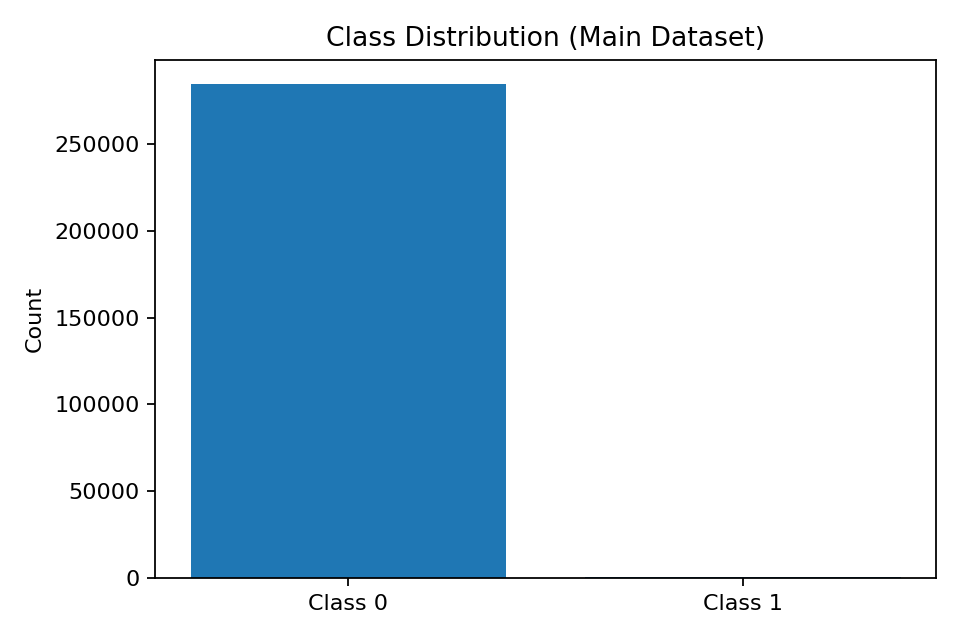
\includegraphics[width=0.72\textwidth]{../outputs/stage1/class_distribution_main.png}
\caption{Class distribution on the main dataset}
\label{fig:stage1_class_dist}
\end{figure}

\begin{figure}[H]
\centering
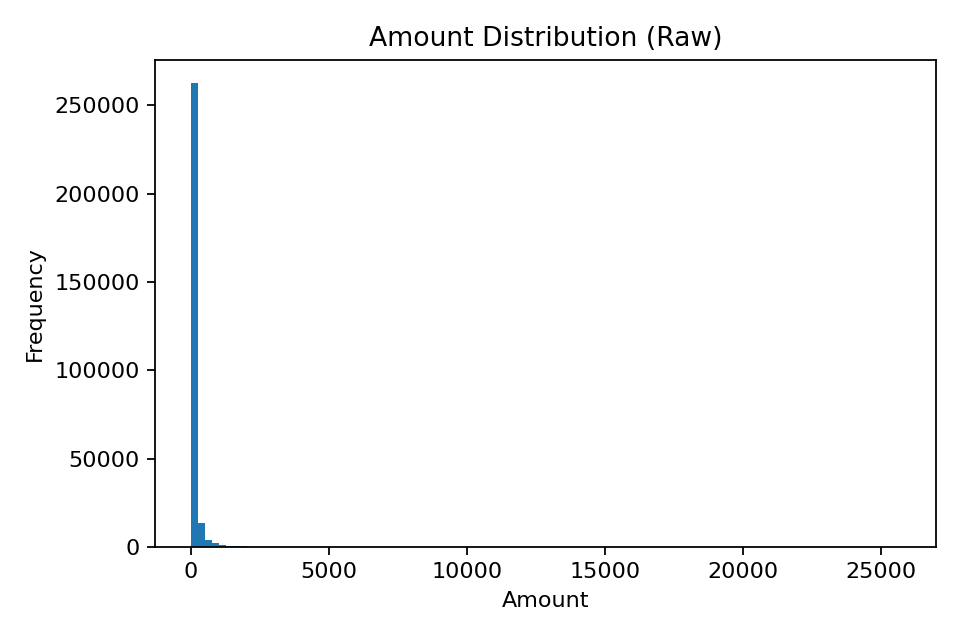
\includegraphics[width=0.72\textwidth]{../outputs/stage1/amount_distribution_main.png}
\caption{Amount distribution on the main dataset}
\label{fig:stage1_amount_dist}
\end{figure}

\subsection{Stage 2 Model Comparison}
\begin{figure}[H]
\centering
\begin{subfigure}{0.31\textwidth}
  \centering
  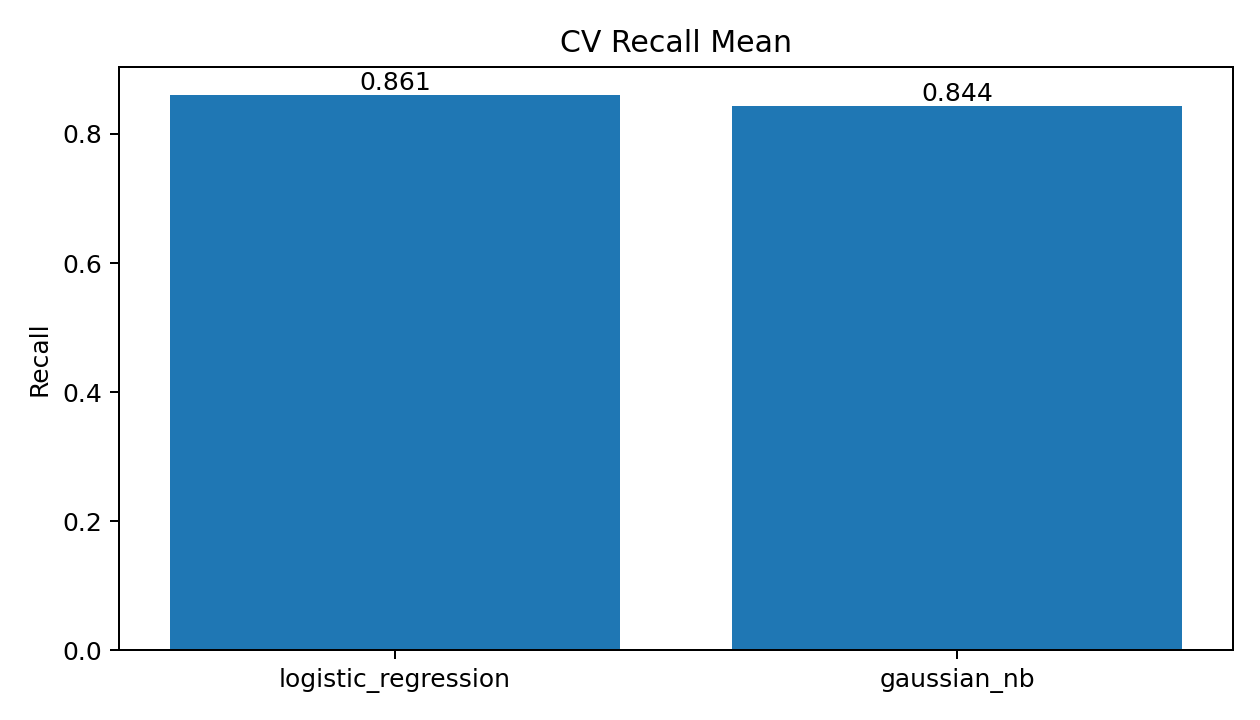
\includegraphics[width=\linewidth]{../outputs/stage2/cv_recall_mean.png}
  \caption{CV Recall}
\end{subfigure}
\hfill
\begin{subfigure}{0.31\textwidth}
  \centering
  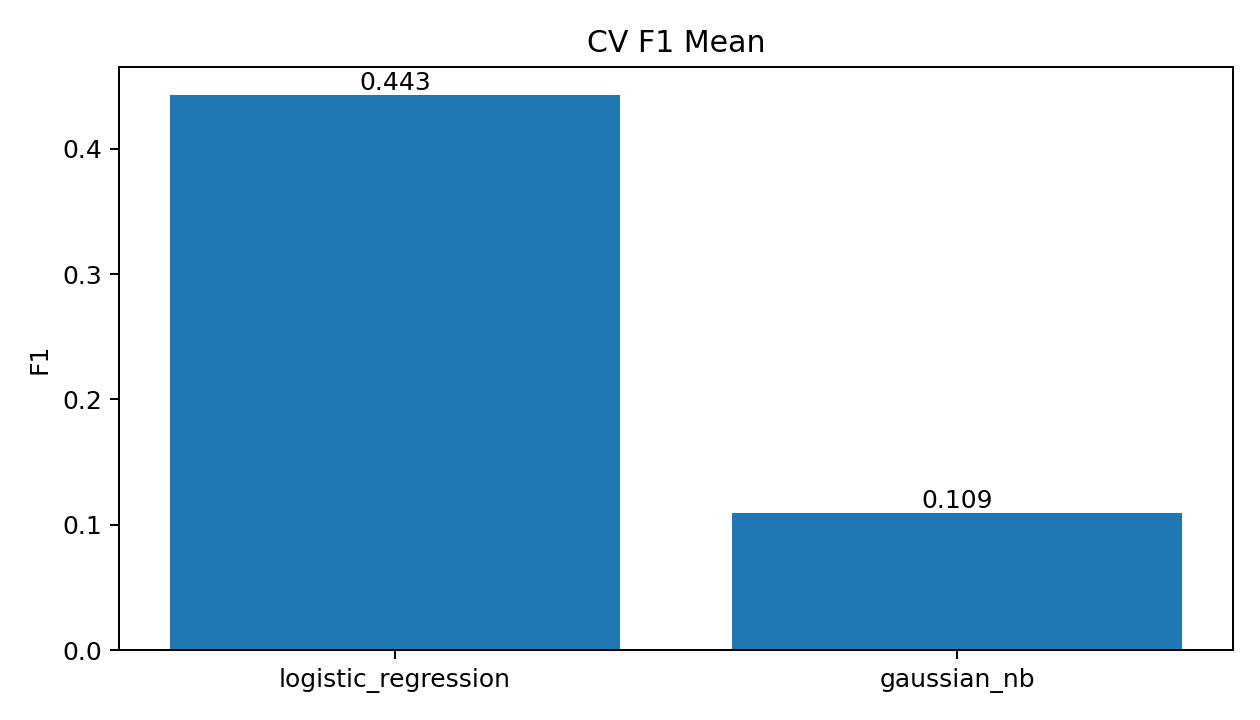
\includegraphics[width=\linewidth]{../outputs/stage2/cv_f1_mean.png}
  \caption{CV F1}
\end{subfigure}
\hfill
\begin{subfigure}{0.31\textwidth}
  \centering
  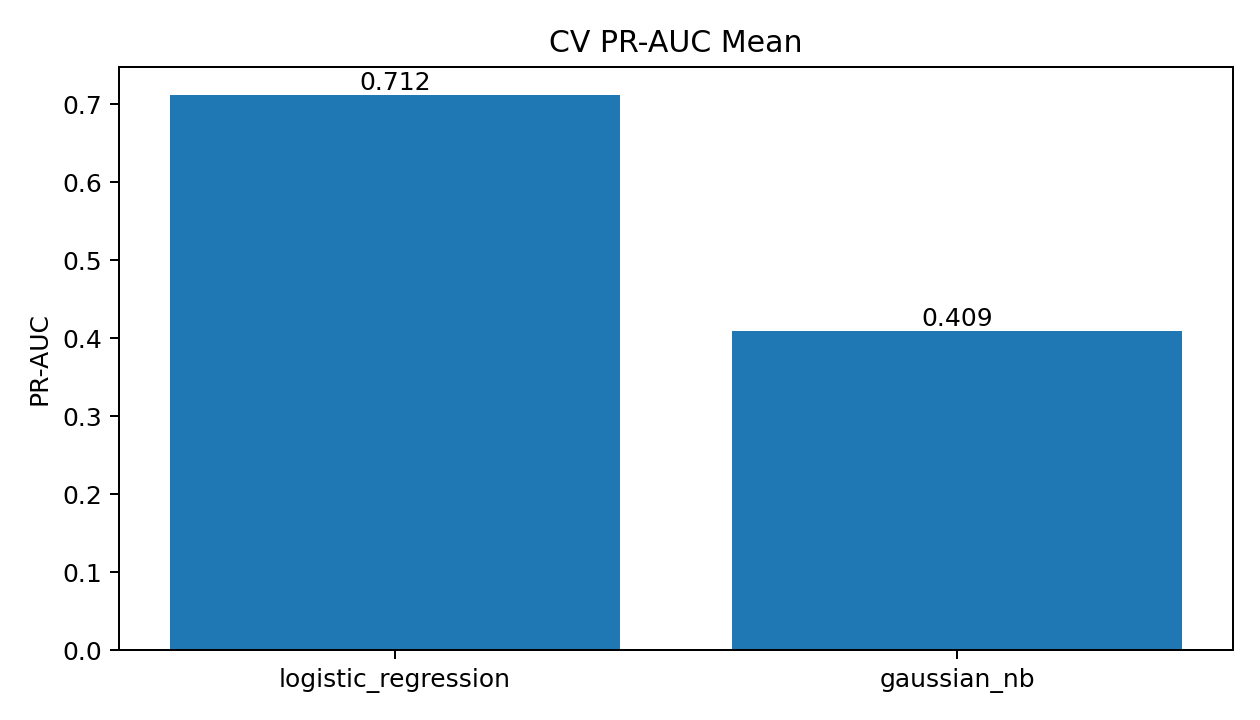
\includegraphics[width=\linewidth]{../outputs/stage2/cv_prauc_mean.png}
  \caption{CV PR-AUC}
\end{subfigure}
\caption{Cross-validation comparison across models}
\label{fig:stage2_cv_comp}
\end{figure}

\begin{figure}[H]
\centering
\begin{subfigure}{0.48\textwidth}
  \centering
  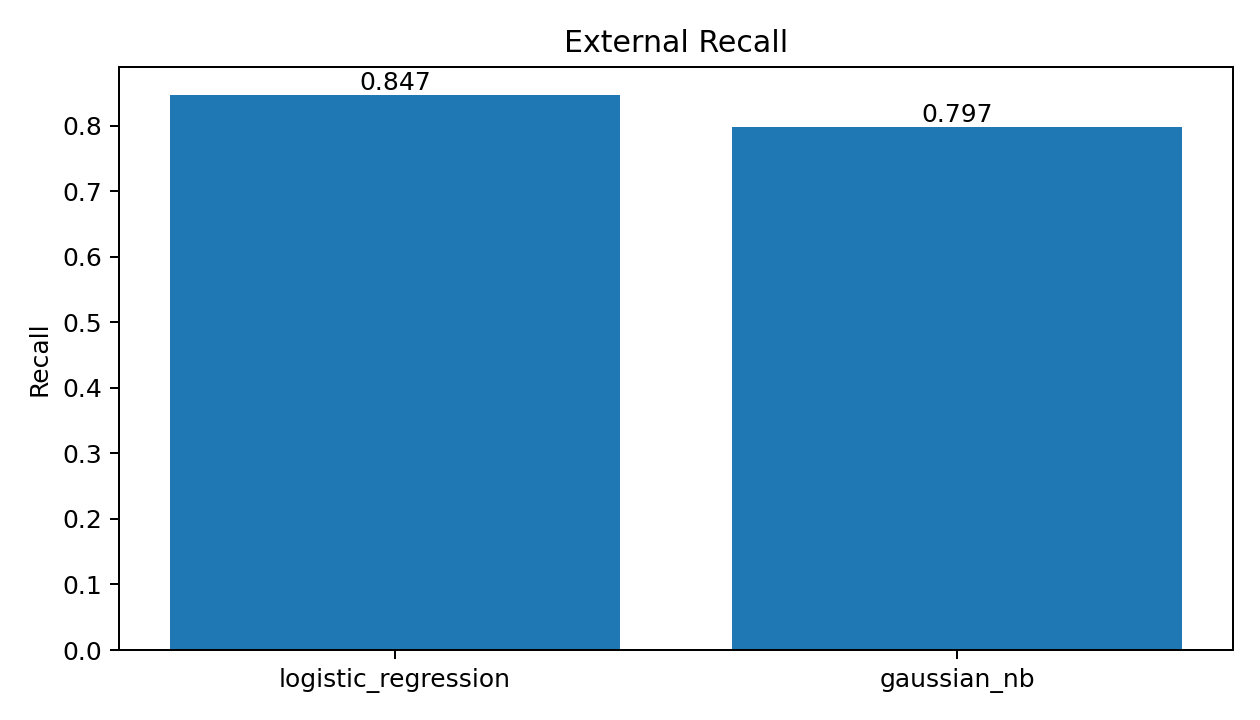
\includegraphics[width=\linewidth]{../outputs/stage2/ext_recall.png}
  \caption{External Recall}
\end{subfigure}
\hfill
\begin{subfigure}{0.48\textwidth}
  \centering
  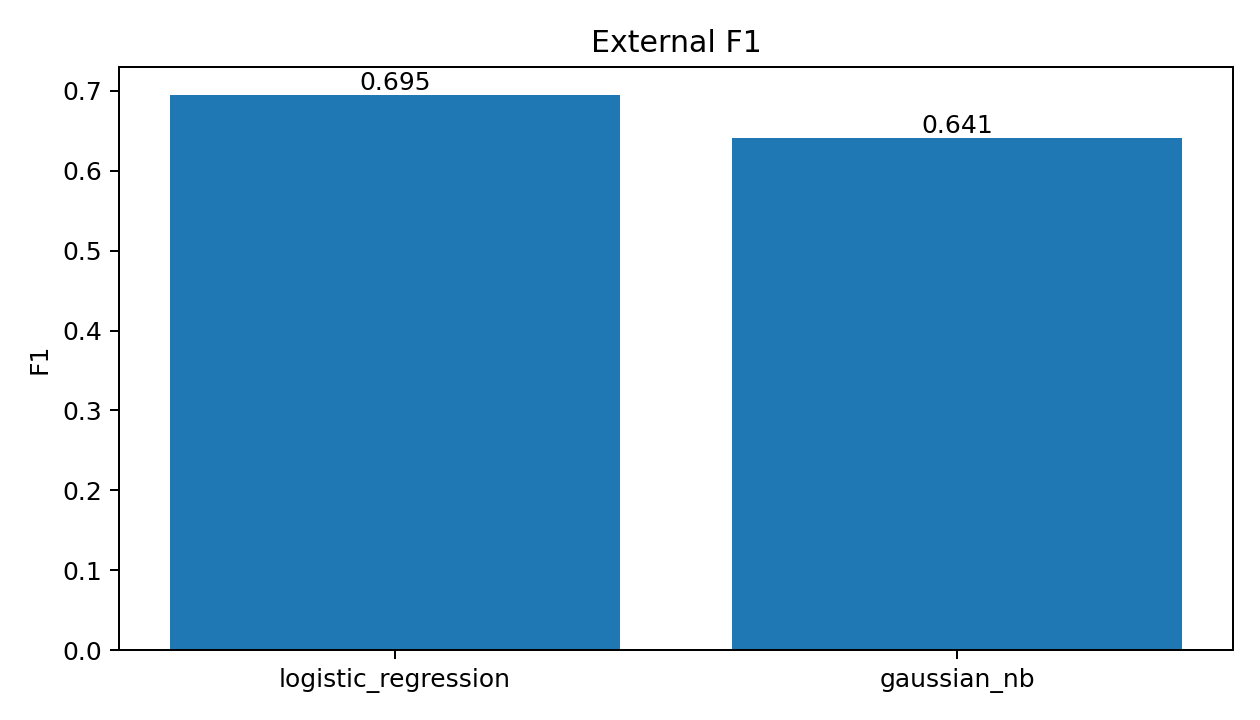
\includegraphics[width=\linewidth]{../outputs/stage2/ext_f1.png}
  \caption{External F1}
\end{subfigure}
\caption{External validation comparison}
\label{fig:stage2_ext_comp}
\end{figure}

\begin{figure}[H]
\centering
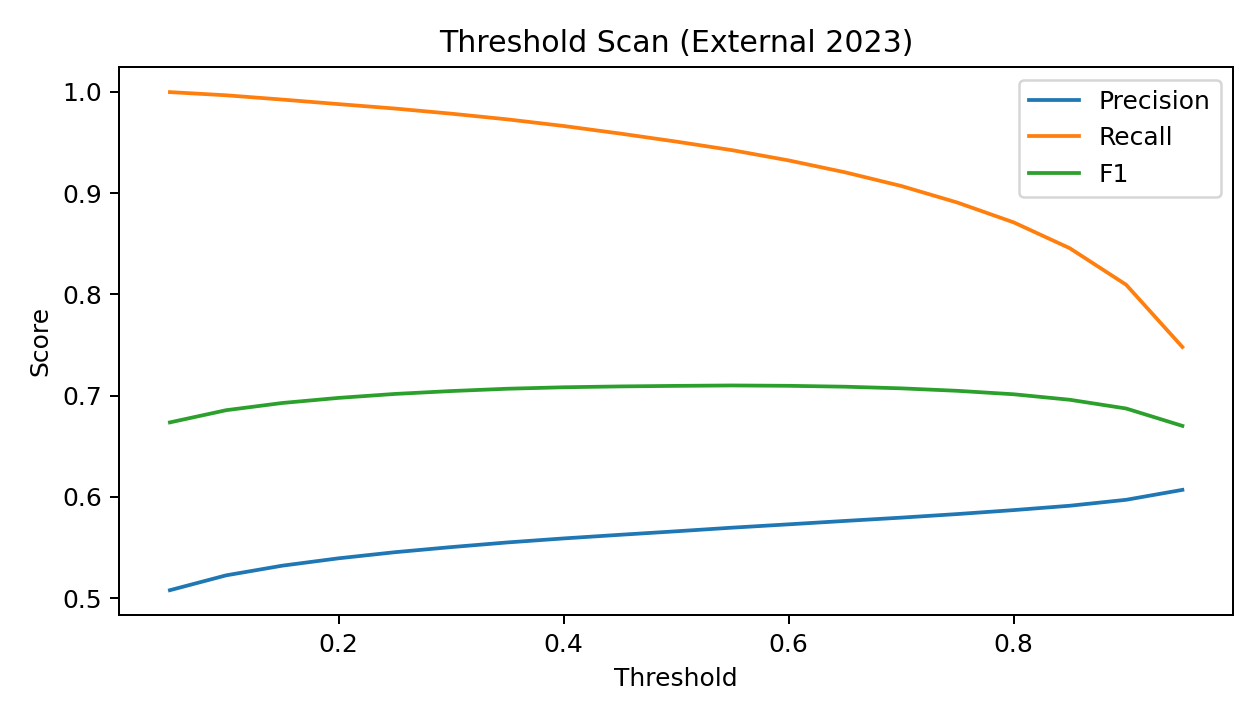
\includegraphics[width=0.72\textwidth]{../outputs/stage2/threshold_scan_ext2023.png}
\caption{Threshold scan on external dataset}
\label{fig:threshold_scan_ext}
\end{figure}

\section{Conclusion and Next Steps}
The current pipeline is reproducible and already includes from-scratch implementation, strict evaluation protocol, cross-validation evidence, external generalization checks, threshold analysis, and ablation experiments. Logistic Regression is selected as the primary model for subsequent optimization.

Next steps include:
\begin{itemize}
  \item finer-grained threshold search (step size < 0.05),
  \item feature-level impact analysis and error-case analysis,
  \item cost-sensitive objective tuning to reduce false-positive cost,
  \item final alignment of report tables/figures and presentation narrative.
\end{itemize}

\section*{Reproducibility Appendix}
Key scripts:
\begin{itemize}
  \item \texttt{scripts/eda\_stage1.py}
  \item \texttt{scripts/prepare\_stage1\_data.py}
  \item \texttt{scripts/models\_from\_scratch.py}
  \item \texttt{scripts/train\_phase2.py}
  \item \texttt{scripts/plot\_phase2\_results.py}
  \item \texttt{scripts/phase2\_advanced\_analysis.py}
\end{itemize}

\end{document}
